% !TeX root = ../main.tex
% Add the above to each chapter to make compiling the PDF easier in some editors.

\chapter{Related Work}\label{chapter:related_work}

\section{Emission Inventories}
Emission inventories are a collection of emission data of pollutants or greenhouse gases (GHGs) released into the atmosphere over a specified period within a defined geographic area.
They serve as foundational tools for environmental management, play a pivotal role in policy formulation, and are crucial for compliance with international agreements on climate change mitigation.
Typically, these inventories are constructed using bottom-up methodologies.
These methods combine individual sources as emissions, providing a comprehensive overview.

The bottom-up approach collects detailed activity data for each emission source, such as fuel consumption rates or industrial production volumes.
Emission factors, representing the average emissions per unit of activity, are then multiplied with these data, resulting in an estimate of the total emissions of that source.
This method makes sectoral analysis possible, thus enabling the identification of crucial emission contributors.

While emission inventories offer detailed estimates, they can be inaccurate due to incomplete data, outdated emission factors, and the exclusion of unknown or hidden emission sources.
These limitations highlight the need for top-down approaches, which use atmospheric measurements to reconstruct emission sources.
Top-down approaches hold the promise of identifying potentially overlooked emitters, enhancing the comprehensiveness of emission inventories.

\section{Atmospheric Inversion}
Top-down approaches formulate the emission estimation problem as an inverse problem, where GHG concentrations measured at ground-based or satellite stations are used to infer the underlying emission fields.
An example of a sensor network doing such measurements is the MUCCnet sensor network.
From these measurements, top-down approaches reconstruct the emission field by applying inversion techniques. 

One such technique is Bayesian inversion.
Bayesian inversion is a technique that updates prior knowledge about emissions using a likelihood function derived from measurement data [Rodgers, 2000; Ganesan et al., 2014].
Prior knowledge refers to information we have about emissions before we incorporate the new measurement data.
However, these methods rely heavily on accurate priors, which can introduce bias when incomplete or incorrect prior information.
In urban areas, where emissions can vary significantly in space and time, such methods may need prior assumptions to provide accurate results.

Recent studies have explored sparse reconstruction techniques, overcoming the above limitations.
These methods assume that emissions are spatially sparse (i.e., only a few significant sources contribute significantly to the total emissions) and use optimization techniques to recover the emission field from a limited set of measurements.
Works by Benisch et al. (2020) and Turner et al. (2016) demonstrated that compressed sensing approaches can be practical for reconstructing urban GHG emissions, especially when combined with sparse priors or transforms, such as wavelets or discrete cosine transforms (DCT).

\section{Compressed Sensing}
Compressed Sensing (CS) is a mathematical framework that enables the recovery of sparse signals from a reduced number of measurements.
The fundamental assumption behind compressed sensing is that the signal of interest is either sparse or compressible in some domain, meaning that most of its components are zero or near zero.
This property allows for the accurate reconstruction of signals even when the number of measurements is significantly smaller than the number of unknowns.

The standard compressed sensing formulation in the context of urban GHG emission estimation is as follows:
\begin{equation}
    y = A x + \epsilon
\end{equation}
where $y \in R$ represents the vector of measurements (e.g., atmospheric GHG concentrations), $A \in R^{m \times n}$ is the sensing matrix that models the relationship between the measurements and the emissions, $x \in R^n$ is the unknown signal (i.e., the emission field), and $\epsilon$ is the noise term, capturing errors or uncertainties in the measurement process.
The sensing matrix $A$ represents the atmospheric transport of molecules and is derived from atmospheric transport models, such as STILT.
Due to a lack of measurements compared to the number of unknowns, this problem is ill-posed.
In urban settings, where emissions are typically sparse, originating from a few dominant sources such as industrial facilities or traffic hubs, compressed sensing provides a natural framework for recovering the emission field from a limited set of observations.

There are many sparse reconstruction algorithms.
One of the most commonly used ones is the Lasso algorithm, which solves the inverse problem by enforcing sparsity through L1-norm regularization.
Another prominent approach is Basis Pursuit (BP), which directly seeks the sparsest solution, and its variant Basis Pursuit with Denoising (BPDN),  which extends the model to handle noisy measurements.
These methods are crucial in emission estimation, where high-dimensional emission fields need to be recovered from a small number of measurements taken by atmospheric sensors.

The Lasso (Least Absolute Shrinkage and Selection Operator) algorithm is a widely used method in compressed sensing due to its ability to enforce sparsity in the solution.
It achieves this by solving the following optimization problem:
\begin{equation}
    \min{\left( \norm{Ax -y }_2^2 + \alpha\norm{x}_1 \right)}
\end{equation}

In this formulation, $\norm{Ax -y }_2^2$ is the least-squares term that measures the difference between the observed measurements $y$ and the predicted measurements $Ax$.
In contrast, the L1-norm $\norm{x}_1$ promotes sparsity.
The parameter $\alpha$ controls the trade-off between the fit's accuracy and the solution's sparsity.
A larger $\alpha$ results in a sparser solution, whereas a smaller $\alpha$ allows for a closer fit to the observed data.
A smaller $\alpha$ may thus introduce non-zero components in $x$, leading to less sparsity.

Basis Pursuit (BP) is another widely adopted algorithm for sparse reconstruction, particularly when the target is to find the sparsest possible solution that satisfies the measurement constraints $y = Ax$ exactly.
Basis pursuit solves the following optimization problem:
\begin{equation}
    \min \norm{x}_1 \quad \text{subject to} \quad  Ax = y
\end{equation}

Here, the objective is to minimize the L1-norm of the signal with the constraint of matching the predicted measurements $A x$ with the observed measurements $y$ exactly.
In contrast to Lasso, basis pursuit does not include a regularization term and instead focuses solely on finding the sparsest solution that satisfies the measurement equation.

Basis pursuit is ideal when the measurement process is noiseless, and the sensing matrix $A$ satisfies the Restricted Isometry Property (RIP), ensuring that different sparse signals remain distinguishable.
However, in real-world applications, such as atmospheric GHG monitoring, measurements are rarely noise-free, and enforcing $Ax = y$ can lead to inaccurate reconstructions when noise is present.

To address the limitations of basis pursuit in noisy environments, Basis Pursuit with Denoising (BPDN) introduces a tolerance for noise in the measurement process.
BPDN modifies the original basis pursuit problem by allowing deviations from the exact measurement equation:
\begin{equation}
 \min \norm{x}_1 \quad \text{subject to} \quad  Ax -y \le \delta
\end{equation}

In this formulation, $\delta$ represents the allowable level of noise or error in the measurements.
Again, the L1-norm is minimized to promote sparsity in the signal, while the L2-norm ensures that the predicted measurements are close to the observed measurements within a defined noise threshold.
The parameter $\delta$ allows BPDN to flexibly handle noisy data, making it more suitable for real-world scenarios, such as urban GHG emission estimation, where measurement noise is inevitable due to sensor inaccuracies and atmospheric variability.

Basis Pursuit with Denoising strikes a balance between sparsity and measurement accuracy. It is beneficial when the sensing matrix $A$ does not fully satisfy RIP, or the measurement process involves significant noise.
By allowing for a controlled level of error, BPDN can recover the sparse emission field without being overly sensitive to noise.
This means that BPDN can tolerate a certain amount of noise in the measurements, ensuring robust solutions.

I should probably add the advantages of Lasso vs BPDN and vice versa.
They can be shown to be quivalent for some $\alpha$, but this also means that Lasso requires tuning of $\alpha$.
However, Lasso is computationally more efficient.
In cases where the computational complexity is not a problem, this thesis will make use of BPDN.

I should also probably put some notes on transformations which makes signal more sparse.

\section{Generative Models for Compressed Sensing}
As mentioned, compressed sensing traditionally assumes that the underlying signals are sparse on some basis.
However, this assumption may only hold in some applications.
For instance, in urban emissions scenarios, while large point sources are often known or can be well-estimated, diffuse or area sources result in emission fields that are less sparse.
This lack of sparsity challenges the effectiveness of conventional compressed sensing techniques, potentially leading to reconstruction failures.

Generative models offer a promising alternative by relaxing the strict sparsity constraint.
These models learn complex representations directly from data, circumventing the need for pre-specified sparse bases.
Recent advancements in fields such as medical imaging have successfully applied generative models to solve compressed sensing problems (cite). %\parencite{jalal2021robust}).

In this thesis, we focus on the pioneering work by Bora et al. (cite), a framework that leverages generative models to improve upon classical compressed sensing techniques.
Their approach demonstrates that using neural networks trained to model the distribution of the underlying data can significantly enhance the performance of compressed sensing.

\subsection{Generative Models}

Bora et al.'s framework primarily involves generative adversarial network (GAN) type models, including Variational Autoencoders (VAEs) and Generative Adversarial Networks (GANs).
Both VAEs and GANs generate samples from lower-dimensional noise, transforming a latent variable $z \in \mathbb{R}^d$ into a data sample $x \in \mathbb{R}^n$ through a generator function $G: \mathbb{R}^d \to \mathbb{R}^n$.

Variational Autoencoders (VAEs) are probabilistic models that encode input data into a latent space and then decode it back to the original space.
They optimize a variational lower bound on the data likelihood, effectively learning a smooth latent space that captures the data distribution.

Generative Adversarial Networks (GANs) consist of two neural networks, a generator $G$ and a discriminator $D$, trained in a minimax game.
The generator tries to produce data that is indistinguishable from real data, while the discriminator attempts to differentiate between real and generated data.
GANs are known for generating high-quality samples but can be challenging to train due to instability in the adversarial objectives.

While GANs often show superior quality in sample generation across various domains, their training instability makes them less suitable for some applications.
Therefore, this thesis chooses VAEs as the appropriate type of generative model due to their stability and structured latent space.

Besides Bora et al. work there are many different approaches (cite the overview).
For example, work using score-based or diffusion models (cite) in the context of medical imaging (cite).
Additionally, normalizing flows (cite) also show promising reults (cite).
But since the goal of this thesis is not to compare individual ML based compressed sensing approaches, the focus lies on Bora et al. work.

\subsection{The Range of a Generator}

The range of a generator $G$ refers to the set of all possible outputs $G(z)$ as $z$ varies over the latent space $\mathbb{R}^d$.
This range represents the subset of the signal space $\mathbb{R}^n$ that the generative model can produce.
In the context of compressed sensing, the reconstruction is constrained to lie within this range, which underscores the importance of the generative model accurately capturing the true data distribution.

\subsection{Compressed Sensing Framework}

Bora et al.'s approach integrates generative models into the compressed sensing reconstruction process.
Given a linear measurement model:
\begin{equation}
 y = A x + \epsilon
\end{equation}
where $A \in \mathbb{R}^{m \times n}$ is the sensing matrix, $x \in \mathbb{R}^n$ is the unknown signal (e.g., an emission field), $y \in \mathbb{R}^m$ represents the measurements, and $\epsilon$ denotes noise, the goal is to recover $x$ from $y$.

The key idea is to leverage a pre-trained generative model $G$ as a prior for $x$.
In contrast to Bayesian inversion, which heavily relies on a predefined prior, which can be a significant limitation if the prior does not accurately reflect the actual spatial distribution of emissions, the prior is more robust.
A generative model would avoid this by learning the prior directly from the data.
The reconstruction problem is formulated as an optimization over the latent space:

\begin{equation}
 \min_{z}{\left( \norm{A G(z) - y}_2^2 + \gls{gamma} R(z) \right)}
\end{equation}
Here, $R(z)$ is a regularization term that encourages desirable properties in the solution, and $\gls{gamma}$ controls the strength of the regularization.
For instance, in the case of $z$ being Gaussian distributed, the regularization $R(z) = \norm{z}_2^2$ can be used, similar to Ridge regression.
The generative model $G$ represents the range of possible signals, and the optimization seeks the latent vector $z$ that, when passed through $G$, produces a signal that matches the measurements $y$ as closely as possible.

Since $G$ is differentiable with respect to $z$, gradient-based optimization methods can be employed to solve the problem.
The optimization seeks the latent vector $z^{\star}$ such that $G(z^{\star})$ best explains the measurements $y$.

\begin{figure}[h!]
    \centering
    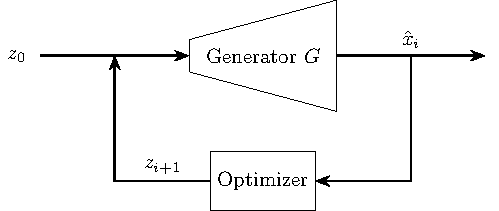
\includegraphics[width=0.75\textwidth]{figures/02_related_work/latent_variable_optimization/build/latent_variable_optimization.pdf}
    \caption{Bora et al paper}
    \label{fig:gen_solver}
\end{figure}

One limitation of Bora et al.'s method is that the reconstructed signal $G(z^{\star})$ is confined strictly to the range of $G$.
This constraint may be too restrictive if $G$ does not perfectly capture the data distribution, leading to reconstruction errors.

Dhar et al. (cite) proposed an extension that allows for sparse deviations from the generator's output to address this issue.
The modified optimization problem introduces an additional variable $s \in \mathbb{R}^n$ representing a sparse offset:

\begin{equation}
 \min_{z, s}{\left(\norm{s}_1 + \gls{lambda} \norm{A \left( G(z) + s \right) - y}_2^2 \right)}
    \label{eq:sparse_deviation}
\end{equation}
where $\norm{s}_1$ promotes sparsity in the offset $s$ and the parameter $\lambda$ balances the sparsity of $s$ with the fit to the measurements $y$.

The reconstructed signal is then given by $\hat{x} = G(z^\star) + s^\star$, where $z^\star$ and $s^\star$ are the solutions to the optimization problem in Equation \ref{eq:sparse_deviation}.

This extension allows the reconstruction to deviate slightly from the generator's range, accommodating components of the signal not captured by $G$, while maintaining overall consistency with the measurements and promoting sparsity in the deviations.

\section{Contributions}
In this work we make the following two assumptions:
\begin{enumerate}
    \item background emissions are known
    \item large emitters are accurately estimated
\end{enumerate}

The point of this work is not to investigate whether compressed sensing theory can be applied in the context of 
This has been investigated by prior work, like Benjis.
The point of this thesis is to investigate whether generative models can be applied.

Is the model able to generalize beyond the trianing data?
Is the model able to reconstruct emitters that are not covered in the emission inventories? 
What is a good dimension for the lower dimensional space?

Mention the rough constributions of this work:
\begin{enumerate}
    \item trained VAE for emission inventories of European cities
    \item demonstrated the applicability of generative models in the context of inverse models for top-down approaches
\end{enumerate}


\section{Contributions}
In this work we make the following two assumptions:
\begin{enumerate}
    \item background emissions are known
    \item large emitters are accurately estimated
\end{enumerate}

The point of this work is not to investigate whether compressed sensing theory can be applied in the context of 
This has been investigated by prior work, like Benjis.
The point of this thesis is to investigate whether generative models can be applied.

Is the model able to generalize beyond the trianing data?
Is the model able to reconstruct emitters that are not covered in the emission inventories? 
What is a good dimension for the lower dimensional space?

Mention the rough constributions of this work:
\begin{enumerate}
    \item trained VAE for emission inventories of European cities
    \item demonstrated the applicability of generative models in the context of inverse models for top-down approaches
\end{enumerate}
